% elementos pré-textuais 

% título do sumário
\ifdefined\contentsname
  \renewcommand*\contentsname{SUMÁRIO}
\else
  \newcommand\contentsname{SUMÁRIO}
\fi

% capa 
\imprimircapa

% folha de rosto 
% o * indica que haverá a ficha bibliográfica 
\imprimirfolhaderosto*

% ficha catalográfica 
%\begin{fichacatalografica}
%    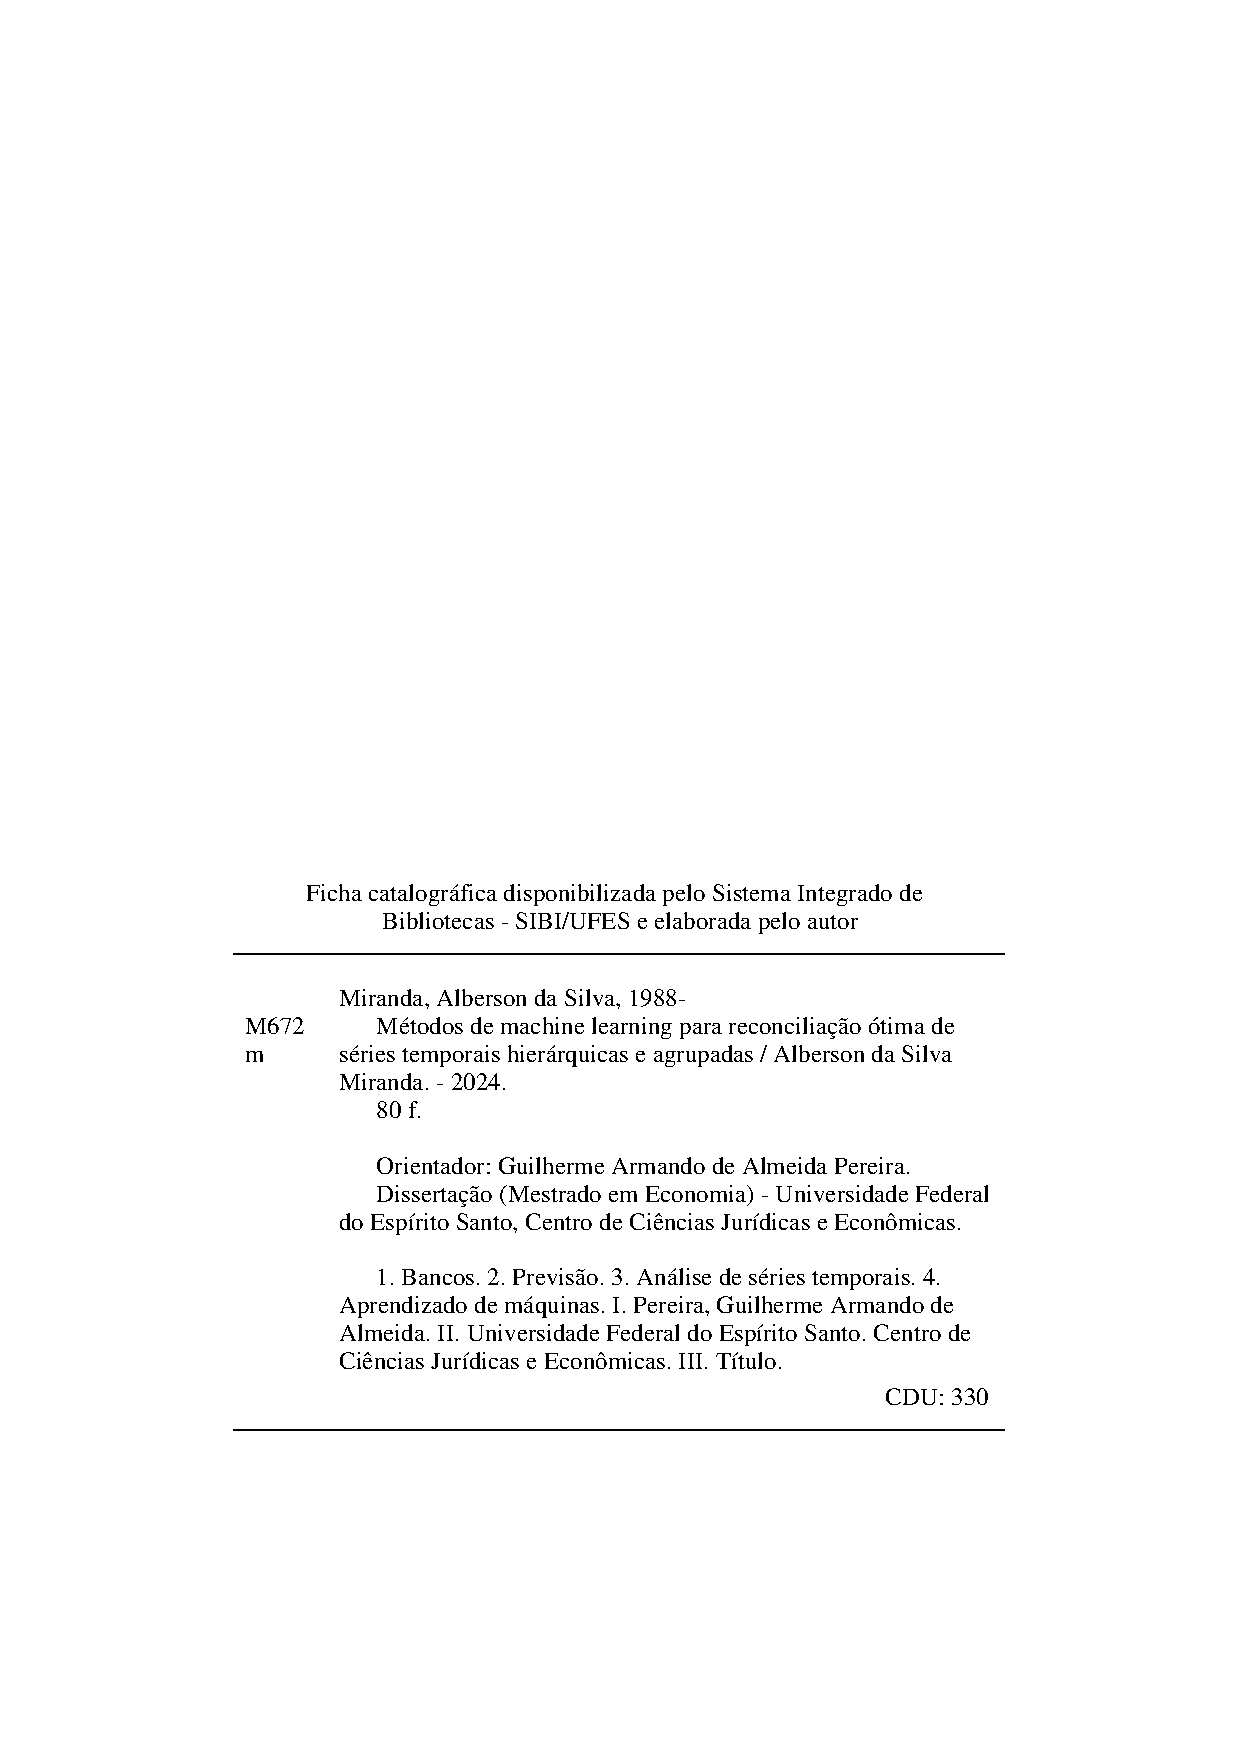
\includepdf{ficha_ufes.pdf}
%\end{fichacatalografica}


% substituir pela ficha em pdf fornecida pela UFES após defesa 
\begin{fichacatalografica}
	\sffamily
	\vspace*{\fill}					% Posição vertical
	\begin{center}					% Minipage Centralizado
	\fbox{\begin{minipage}[c][8cm]{15cm}		% Largura
	\small
	\imprimirautor
	
	\hspace{0.5cm} \imprimirtitulo  / \imprimirautor. --
	\imprimirlocal, \imprimirdata-
	
	\hspace{0.5cm} \thelastpage p. : il. (algumas color.) ; 30 cm.\\
	
	\hspace{0.5cm} \imprimirorientadorRotulo~\imprimirorientador\\
	
	\hspace{0.5cm}
	\parbox[t]{\textwidth}{\imprimirtipotrabalho~--~\imprimirinstituicao,
	\imprimirdata.}\\
	
	\hspace{0.5cm}
		1. Economia Bancária.
		2. Séries Temporais Hierárquicas.
		3. Reconciliação Ótima.
    4. Machine Learning.
		I. Pereira, Guilherme Armando de Almeida.
		II. Universidade Federal do Espírito Santo.
		III. Centro de Ciências Jurídicas e Econômicas.
		IV. Título 			
	\end{minipage}}
	\end{center}
\end{fichacatalografica}

% folha de aprovação 
%
%\begin{folhadeaprovacao}
%    \includepdf{folhadeaprovacao_final.pdf}
%\end{folhadeaprovacao}


% substituir pela folha assinada pela banca após defesa 
\begin{folhadeaprovacao}

  \begin{center}
    {\ABNTEXchapterfont\large\imprimirautor}

    \vspace*{\fill}\vspace*{\fill}
    \begin{center}
      \ABNTEXchapterfont\bfseries\Large\imprimirtitulo
    \end{center}
    \vspace*{\fill}
    
    \hspace{.45\textwidth}
    \begin{minipage}{.5\textwidth}
        \imprimirpreambulo
        \vspace*{1cm}
        Aprovada em 29 de fevereiro de 2024.\\[2cm]
        \textbf{COMISSÃO EXAMINADORA} \\
        \assinatura{\textbf{\imprimirorientador} \\ Universidade Federal do Espírito Santo \\ Orientador} 
        \assinatura{\textbf{Prof. Dr. Edson Zambon Monte} \\ Universidade Federal do Espírito Santo}
        \assinatura{\textbf{Prof. Dr. Fernando Luiz Cyrino Oliveira} \\ PUC-Rio}
        %\assinatura{\textbf{Professor} \\ Convidado 3}
        %\assinatura{\textbf{Professor} \\ Convidado 4}
    \end{minipage}%
   \end{center}
  
\end{folhadeaprovacao}

%% dedicatória 
%\begin{dedicatoria}
%   \vspace*{\fill}
%   \centering
%   \noindent
%   \textit{Exemplo de dedicatória,\\\lipsum[10].} \vspace*{\fill}
%\end{dedicatoria}

%% agradecimentos 
%\begin{agradecimentos}
%\lipsum[30]
%
%\lipsum[30]
%
%\end{agradecimentos}

% epígrafe 
%\begin{epigrafe}
%    \vspace*{\fill}
%	\begin{flushright}
%		\textit{``Modelo de epígrafe, \\
%		modelo de epígrafe.''}
%	\end{flushright}
%\end{epigrafe}

% resumo 

\setlength{\absparsep}{18pt}
\begin{resumo}
  Neste estudo, foram conduzidos experimentos de reconciliação ótima de séries temporais e agrupadas para aprimorar a precisão preditiva dos saldos de empréstimos e financiamentos do Banco do Estado do Espírito Santo. Além dos métodos analíticos tradicionais, a investigação explorou abordagens de \textit{machine learning}, incluindo floresta aleatória, \textit{gradient boosting}, \textit{elastic net} e \textit{support vector machines}. A partir da metodologia delineada por \textcite{spiliotis_hierarchical_2021}, o trabalho propôs duas estratégias alternativas para a reconciliação ótima baseada em \textit{machine learning}. Os resultados revelaram que a escolha do método e estratégia depende do nível hierárquico, onde a combinação correta pode exibir até 91\% de ganho de performance nos níveis mais agregados. No entanto, para níveis inferiores, os métodos analíticos, destacadamente o MinT-\textit{Shrink}, foram mais eficazes.

  \textbf{Palavras-chave}: Economia Bancária. Séries Temporais Hierárquicas. Reconciliação Ótima. \textit{Machine Learning}.
\end{resumo}

% abstract 
\begin{resumo}[Abstract]
  \begin{otherlanguage*}{english}
    
In this research, optimal reconciliation experiments were conducted to enhance the predictive accuracy of loan balances at the Bank of the State of Espírito Santo, focusing on hierarchical and grouped time series. In addition to conventional analytical methods, our investigation delved into machine learning approaches, encompassing random forest, gradient boosting, elastic net, and support vector machines. Following the methodology outlined by \textcite{spiliotis_hierarchical_2021}, our work proposed two alternative strategies for optimal reconciliation through machine learning methods. The outcomes underscored the significance of tailoring the method and strategy based on the hierarchical level. The right combination exhibited a remarkable performance improvement of up to 91\% at the most aggregated levels. Notably, for lower levels, analytical methods, particularly MinT-Shrink, proved to be more effective.
    \vspace{\onelineskip}
 
    \noindent 
    \textbf{Keywords}: Economics of Banking. Hierarchical Time-Series. Optimal Reconciliation. Machine Learning.
  \end{otherlanguage*}
\end{resumo}

% lista de ilustrações 
\pdfbookmark[0]{\listfigurename}{lof}
\listoffigures*
\cleardoublepage

% lista de quadros 
%\pdfbookmark[0]{\listofquadrosname}{loq}
%\listofquadros*
%\cleardoublepage

% lista de tabelas 
\pdfbookmark[0]{\listtablename}{lot}
\listoftables*
\cleardoublepage

% lista de abreviaturas 
\begin{siglas}
  \item[ETS] \textit{Exponentional Smoothing}
  \item[Favar] \textit{Factor Augmented Vector Autoregression}
  \item[Lasso] \textit{Least Absolute Shrinkage and Selection Operator}
  \item[MCRL] Modelo Clássico de Regressão Linear
  \item[MASE] \textit{Mean Absolute Scaled Error}
  \item[MinT] \textit{Minimum Trace}
  \item[MQGF] Mínimos Quadrados Generalizados Factíveis
  \item[MQO] Mínimos Quadrados Ordinários
  \item[MQP] Mínimos Quadrados Ponderados
  \item[PIB] Produto Interno Bruto
  \item[RMSSE] \textit{Root Mean Squared Scaled Error}
  \item[SFN] Sistema Financeiro Nacional
  \item[SVR] \textit{Support Vector Regression}
  \item[XGBoost] \textit{Extreme Gradient Boosting}
\end{siglas}

% lista de símbolos 
\begin{simbolos}
  \item[$ t $] Tempo dentro da amostra
  \item[$ T $] Último tempo dentro da amostra
  \item[$ h $] Horizonte de previsão, tempo fora da amostra
  \item[$ \Omega $] Conjunto de dados dentro da amostra
  \item[$ y $] Série temporal dentro da amostra
  \item[$ \hat{y} $] Série temporal estimada
  \item[$ \tilde{y} $] Série temporal reconciliada
  \item[$ n $] Número de séries na hierarquia
  \item[$ m $] Número de séries no menor nível da hierarquia
  \item[$ k $] Número de níveis na hierarquia
  \item[$ \mathbfit{S} $] Matriz de soma
  \item[$ \mathbfit{G} $] Matriz de reconciliação
  \item[$\{...\}$] Conjunto
  \item[$|\{...\}|$] Cardinalidade de um conjunto
\end{simbolos}

% sumário 
\pdfbookmark[0]{\contentsname}{toc}
\tableofcontents*
\cleardoublepage

% elementos textuais 
\textual
\pagestyle{simple}